\chapter{Arhitektura i dizajn sustava}
		

		Arhitekturu web aplikacije dijelimo na tri podsustava:
		\begin{itemize}
			\item Web aplikacija
			\item Web poslužitelj
			\item Baza podataka
		\end{itemize}
	
		\begin{figure}[H]
			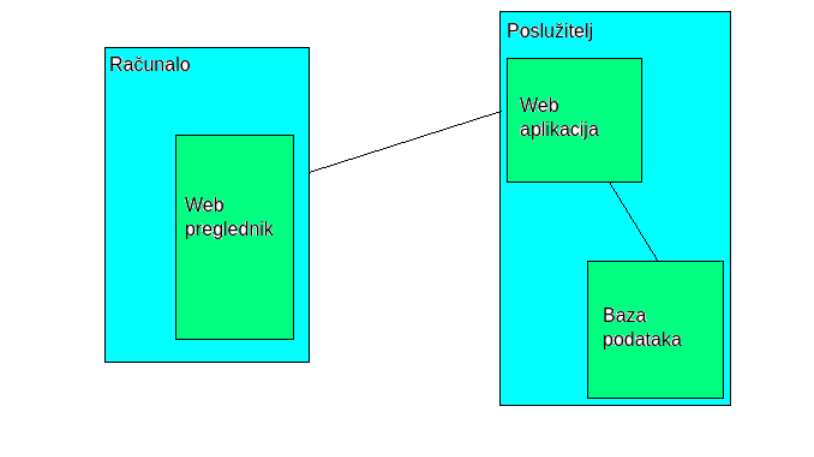
\includegraphics[width=\textwidth]{slike/arhitektura.png}
			\centering
			\caption{Arhitektura sustava}
			\label{fig:arhitektura_sustava}
		\end{figure}
	
		\underline{\textit{Web preglednik}} (eng. \textit{web browser}) je korisnički program koji omogućuje pregledavanje statičkih i dinamičkih sadržaja interneta. Web preglednik dohvaća sadržaj s lokalnog ili udaljenog računala, i potom taj sadržaj interpretira i prikazuje korisniku. Neki od popularnijih web preglednika današnjice su Chrome, Safari, Firefox i Edge.
		
		\underline{\textit{Web poslužitelj}} (eng. \textit{web server}) je temelj aplikacije, a služi za komunikaciju. Korisnik i aplikacija razmjenjuju HTTP zahtjeve (eng. \textit{HTTP request}) i HTTP odgovore (eng. \textit{HTTP response}). Poslužitelj pokreće prednji kraj (eng. \textit{front end}) i stražnji kraj (eng. \textit{back end}). Radi jednostavnosti, baza podataka je također smještena na poslužitelju.
		
		Korisnik kroz grafičko sučelje, odnosno prednji kraj, šalje zahtjeve na REST pristupne točke stražnjeg kraja. Tada stražnji kraj procesuira zahtjev i ako je potrebno komunicira s bazom podataka. Nakon konstrukcije, stražnji kraj šalje odgovor prednjem kraju u obliku JSON objekta, a prednji kraj procesuira odgovor i promjene prikazuje korisniku u obliku HTML stranice. 
		
		Za aplikaciju je odabrana višeslojna arhitektura temeljena na \textbf{MVC} (\textit{model-view-controller}) arhitekturnom stilu te uslužnoj arhitekturi.
		
		\begin{enumerate}
			\item \textit{sloj korisničke strane} - korisničko sučelje implementirano u JavaScriptu i radnom okviru AngularJS
			\item \textit{sloj nadglednika} - REST nadglednici 
			\item \textit{sloj domene} - model podataka iz domene primjene
			\item \textit{sloj za pristup podacima} - posrednik između sloja domene i baze podataka
			\item \textit{sloj baze podataka} - pohrana podataka
		\end{enumerate}
		
		Ovakva arhitektura odabrana je zbog poželjnih svojstava MVC arhitekturnog stila i višeslojne arhitekture: razvoj pojedinih slojeva jednostavniji je i u velikom stupnju nezavisan od razvoja drugih slojeva. Također, komunikacija prednjeg i stražnjeg kraja je ostvarena primjenom REST arhitketurnog stila. Zbog toga su prednji i stražnji kraj neovisni u smislu jezika implementacije, što potiče ponovnu uporabu.
		
		MVC arhitekturni stil sastoji se od tri koncepta:
		\begin{itemize}
			\item \textbf{Model} - reprezentacija strukture podataka koja se koristi u rješenju, neovisna o korisničkom sučeju
			\item \textbf{View} - pogled na podatke, u našoj aplikaciji to je grafičko sučelje
			\item \textbf{Controller} - nadzornik koji koordinira zahtjeve i odgovore između modela i pogleda, sadrži svu logiku upravljanja.
		\end{itemize}
				
		\section{Baza podataka}
			
			Za našu web aplikaciju koristimo PostgreSQL relacijsku bazu podataka. Pogodna je jer ima široku korisničku podršku, dokazanu stabilnost, dostupnost sučelja s Javom, a i već smo upoznati s njom iz prijašnjih iskustva. Relacijska baza podataka omogućuje jednostavno modeliranje problema domene, a temeljna joj je zadaća sigurna i brza pohrana i dohvat podataka. Temeljna građevna jedinica baze podataka je relacija, odnosno tablica. Jedna tablica predstavlja jedan entitet, a naša baza sastoji se od ovih relacija :
		
			\begin{itemize}
				\item user
				\item media
				\item pets
				\item posts
				\item comments
				\item relationships
				\item events
				\item event responses
				\item event comments
				\item company services
				\item company info
				\item messages
				\item reports
				\item blocks
			\end{itemize}
		
			\subsection{Opis tablica}
				
				\textbf{user} - Ovaj entitet predstavlja korisnika. Sadrži atribute ID, korisničko ime, lozinka, ime, prezime, email, tip korisnika, uloga korisnika, ID profilne slike.
				
				\begin{longtblr}[
					label=none,
					entry=none
					]{
						width = \textwidth,
						colspec={|X[8,l]|X[6, l]|X[20, l]|}, 
						rowhead = 1,
					} %definicija širine tablice, širine stupaca, poravnanje i broja redaka naslova tablice
					\hline \multicolumn{3}{|c|}{\textbf{user}}	 \\ \hline[3pt]
					\SetCell{LightGreen}id & SERIAL	& jedinstveni identifikator korisnika  	\\ \hline
					username & VARCHAR & korisničko ime  	\\ \hline 
					password & VARCHAR & korisnička lozinka \\ \hline 
					first\_name & VARCHAR & ime korisnika		\\ \hline 
					last\_name & VARCHAR & prezime korisnika		\\ \hline
					email & VARCHAR & korisnikov email			\\ \hline
					user\_type & ENUM & tip korisnika		\\ \hline
					user\_role & ENUM & uloga korisnika		\\ \hline
					\SetCell{LightBlue} profile\_picture\_id & BIGINT & id korisničke slike	\\ \hline
				\end{longtblr}
				
				\textbf{media} - Ovaj entitet predstavlja medijski sadržaj. Sadrži atribute ID i sam medijski sadržaj.
			
				\begin{longtblr}[
					label=none,
					entry=none
					]{
						width = \textwidth,
						colspec={|X[8,l]|X[6, l]|X[20, l]|}, 
						rowhead = 1,
					} %definicija širine tablice, širine stupaca, poravnanje i broja redaka naslova tablice
					\hline \multicolumn{3}{|c|}{\textbf{media}}	 \\ \hline[3pt]
					\SetCell{LightGreen}id & BIGSERIAL	& jedinstveni identifikator sadržaja   \\ \hline
					content & BYTEA & sadržaj  	\\ \hline 
				\end{longtblr}
				
				\textbf{pets} - Ovaj entitet predstavlja kućnog ljubimca. Sadrži atribute ID, tip ljubimca, ime, vlasnik, dob, spol, ID profilne slike, opis, pasmina.
				
				\begin{longtblr}[
					label=none,
					entry=none
					]{
						width = \textwidth,
						colspec={|X[8,l]|X[6, l]|X[20, l]|}, 
						rowhead = 1,
					} %definicija širine tablice, širine stupaca, poravnanje i broja redaka naslova tablice
					\hline \multicolumn{3}{|c|}{\textbf{pets}}	 \\ \hline[3pt]
					\SetCell{LightGreen}id & BIGSERIAL	& jedinstveni identifikator ljubimca  	\\ \hline
					type & ENUM & tip životinje  	\\ \hline 
					name & VARCHAR & ime ljubimca  	\\ \hline 
					age & INT & dob ljubimca		\\ \hline 
					gender & ENUM & spol ljubimca		\\ \hline
					description & VARCHAR & opis ljubimca		\\ \hline
					breed & VARCHAR & pasmina		\\ \hline
					\SetCell{LightBlue} owner & BIGINT & id vlasnika ljubimca \\ \hline 
					\SetCell{LightBlue} profile\_picture\_id & BIGINT & id korisničke slike	\\ \hline
				\end{longtblr}
			
				\textbf{posts} - Ovaj entitet predstavlja objavu. Sadrži atribute ID, ID korisnika, ID sadržaja i opis, odnosno samu objavu.
				
				\begin{longtblr}[
					label=none,
					entry=none
					]{
						width = \textwidth,
						colspec={|X[8,l]|X[6, l]|X[20, l]|}, 
						rowhead = 1,
					} %definicija širine tablice, širine stupaca, poravnanje i broja redaka naslova tablice
					\hline \multicolumn{3}{|c|}{\textbf{posts}}	 \\ \hline[3pt]
					\SetCell{LightGreen}id & BIGSERIAL	& jedinstveni identifikator objave 	\\ \hline
					\SetCell{LightBlue} user\_id & BIGINT & id korisnika koji objavljuje 	\\ \hline 
					\SetCell{LightBlue} content\_id & BIGINT & id medijskog sadržaja \\ \hline 
					description & VARCHAR & sadržaj objave		\\ \hline 
				\end{longtblr}
			
				\textbf{comments} - Ovaj entitet predstavlja komentar na objavu. Sadrži atribute ID, ID korisnika, ID objave i sadržaj, odnosno komentar.
				
				\begin{longtblr}[
					label=none,
					entry=none
					]{
						width = \textwidth,
						colspec={|X[8,l]|X[6, l]|X[20, l]|}, 
						rowhead = 1,
					} %definicija širine tablice, širine stupaca, poravnanje i broja redaka naslova tablice
					\hline \multicolumn{3}{|c|}{\textbf{comments}}	 \\ \hline[3pt]
					\SetCell{LightGreen}id & BIGSERIAL	& jedinstveni identifikator objave 	\\ \hline
					\SetCell{LightBlue} user\_id & BIGINT & id korisnika koji objavljuje komentar 	\\ \hline 
					\SetCell{LightBlue} post\_id & BIGINT & id objave na koju se komentira \\ \hline 
					content & VARCHAR & sadržaj komentara		\\ \hline 
				\end{longtblr}
			
				\textbf{relationships} - Ovaj entitet predstavlja odnose između dva korisnika. Sadrži atribute prvi korisnik, drugi korisnik, tip odnosa između njih.
				
				\begin{longtblr}[
					label=none,
					entry=none
					]{
						width = \textwidth,
						colspec={|X[8,l]|X[6, l]|X[20, l]|}, 
						rowhead = 1,
					} %definicija širine tablice, širine stupaca, poravnanje i broja redaka naslova tablice
					\hline \multicolumn{3}{|c|}{\textbf{relationships}}	 \\ \hline[3pt]
					\SetCell{LightBlue} first\_user & BIGINT & id prvog korisnika		\\ \hline 
					\SetCell{LightBlue} second\_user & BIGINT & id drugog korisnika		\\ \hline
					type & ENUM & tip odnosa između dva korisnika		\\ \hline
				\end{longtblr}
			
				\textbf{events} - Ovaj entitet predstavlja događaje. Sadrži atribute id, organizator, početak, trajanje, opis, lokacija, vidljivost.
				
				\begin{longtblr}[
					label=none,
					entry=none
					]{
						width = \textwidth,
						colspec={|X[8,l]|X[6, l]|X[20, l]|}, 
						rowhead = 1,
					} %definicija širine tablice, širine stupaca, poravnanje i broja redaka naslova tablice
					\hline \multicolumn{3}{|c|}{\textbf{events}}	 \\ \hline[3pt]
					\SetCell{LightGreen}id & BIGSERIAL	& jedinstveni identifikator događaja  	\\ \hline
					\SetCell{LightBlue} organizer & BIGINT & id korisnika organizatora  	\\ \hline 
					start\_date & TIMESTAMP & vrijeme i datum početka događaja	\\ \hline 
					duration & INTERVAL & trajanje događaja \\ \hline 
					description & VARCHAR & opis događaja		\\ \hline
					location & VARCHAR & lokacija događaja			\\ \hline
					visibility & ENUM & vidljivost događaja		\\ \hline
				\end{longtblr}
			
				\textbf{event\_responses} - Ovaj entitet predstavlja odgovore na događaje. Sadrži atribute ID događaja, ID korisnika, odgovor na događaj.
				
				\begin{longtblr}[
					label=none,
					entry=none
					]{
						width = \textwidth,
						colspec={|X[8,l]|X[6, l]|X[20, l]|}, 
						rowhead = 1,
					} %definicija širine tablice, širine stupaca, poravnanje i broja redaka naslova tablice
					\hline \multicolumn{3}{|c|}{\textbf{event\_responses}}	 \\ \hline[3pt]
					\SetCell{LightBlue}event\_id & BIGINT & id događaja 		\\ \hline
					\SetCell{LightBlue}user\_id & BIGINT & id korisnika		\\ \hline
					response & ENUM & odgovor o dolasku	\\ \hline
				\end{longtblr}
				
				\textbf{event\_comments} - Ovaj entitet predstavlja komentare na događaj. Sadrži atribute ID, ID događaja, ID korisnika, komentar.
				
				\begin{longtblr}[
					label=none,
					entry=none
					]{
						width = \textwidth,
						colspec={|X[8,l]|X[6, l]|X[20, l]|}, 
						rowhead = 1,
					} %definicija širine tablice, širine stupaca, poravnanje i broja redaka naslova tablice
					\hline \multicolumn{3}{|c|}{\textbf{event\_comments}}	 \\ \hline[3pt]
					\SetCell{LightGreen} id & BIGSERIAL & jedinstveni identifikator komentara	\\ \hline
					\SetCell{LightBlue}event\_id & BIGINT & id događaja 		\\ \hline
					\SetCell{LightBlue}user\_id & BIGINT & id korisnika		\\ \hline
					content & VARCHAR & sadržaj komentara	\\ \hline
				\end{longtblr}
			
				\textbf{company\_services} - Ovaj entitet predstavlja uslugu koju pruža neka tvrtka. Sadrži atribute ID tvrtke, tip usluge, opis usluge.
				
				\begin{longtblr}[
					label=none,
					entry=none
					]{
						width = \textwidth,
						colspec={|X[8,l]|X[6, l]|X[20, l]|}, 
						rowhead = 1,
					} %definicija širine tablice, širine stupaca, poravnanje i broja redaka naslova tablice
					\hline \multicolumn{3}{|c|}{\textbf{company\_services}}	 \\ \hline[3pt]
					\SetCell{LightBlue}company\_id & BIGINT & jedinstveni identifikator tvrtke	\\ \hline
					service\_type & ENUM & vrsta usluge 		\\ \hline
					service\_description & VARCHAR & opis usluge		\\ \hline
				\end{longtblr}
			
				\textbf{company\_info} - Ovaj entitet predstavlja opis tvrtke. Sadrži atribute ID tvrtke, ime, adresa, kontakt.
				
				\begin{longtblr}[
					label=none,
					entry=none
					]{
						width = \textwidth,
						colspec={|X[8,l]|X[6, l]|X[20, l]|}, 
						rowhead = 1,
					} %definicija širine tablice, širine stupaca, poravnanje i broja redaka naslova tablice
					\hline \multicolumn{3}{|c|}{\textbf{company\_info}}	 \\ \hline[3pt]
					\SetCell{LightBlue}company\_id & BIGINT & jedinstveni identifikator tvrtke		\\ \hline
					name & VARCHAR & ime tvrtke		\\ \hline
					adress & VARCHAR & adresa tvrtke		\\ \hline
					contact & VARCHAR & kontakt tvrtke		\\ \hline
				\end{longtblr}
			
				\textbf{messages} - Ovaj entitet predstavlja poruke između korisnika. Sadrži atribute ID, pošiljatelj, primatelj, sadržaj.
				
				\begin{longtblr}[
					label=none,
					entry=none
					]{
						width = \textwidth,
						colspec={|X[8,l]|X[6, l]|X[20, l]|}, 
						rowhead = 1,
					} %definicija širine tablice, širine stupaca, poravnanje i broja redaka naslova tablice
					\hline \multicolumn{3}{|c|}{\textbf{messages}}	 \\ \hline[3pt]
					\SetCell{LightGreen} id & BIGSERIAL & id događaja 		\\ \hline
					\SetCell{LightBlue}sender & BIGINT & id pošiljatelja		\\ \hline
					\SetCell{LightBlue}receiver & BIGINT & id primatelja		\\ \hline
					content & VARCHAR & sadržaj poruke	\\ \hline
				\end{longtblr}
				
				\textbf{reports} - Ovaj entitet predstavlja prijavu nekog korisnika. Sadrži atribute ID korisnika koji prijavljuje, ID korisnika koji je prijavljen, opis, ID objave, ID poruke, ID komentara.
				
				\begin{longtblr}[
					label=none,
					entry=none
					]{
						width = \textwidth,
						colspec={|X[8,l]|X[6, l]|X[20, l]|}, 
						rowhead = 1,
					} %definicija širine tablice, širine stupaca, poravnanje i broja redaka naslova tablice
					\hline \multicolumn{3}{|c|}{\textbf{reports}}	 \\ \hline[3pt]
					\SetCell{LightBlue}reporter\_id & BIGINT & id korisnika koji prijavljuje		\\ \hline
					\SetCell{LightBlue}reported\_user & BIGINT & id korisnika koji je prijavljen		\\ \hline
					description & VARCHAR & opis prijave	\\ \hline
					\SetCell{LightBlue}post\_id & BIGINT & id objave		\\ \hline
					\SetCell{LightBlue}message\_id & BIGINT & id poruke		\\ \hline
					\SetCell{LightBlue}comment\_id & BIGINT & id komentara	\\ \hline	
				\end{longtblr}
			
				\textbf{blocks} - Ovaj entitet predstavlja blokiranje korisnika. Sadrži atribute ID korisnika, datum odblokiranja.
				
				\begin{longtblr}[
					label=none,
					entry=none
					]{
						width = \textwidth,
						colspec={|X[8,l]|X[6, l]|X[20, l]|}, 
						rowhead = 1,
					} %definicija širine tablice, širine stupaca, poravnanje i broja redaka naslova tablice
					\hline \multicolumn{3}{|c|}{\textbf{blocks}}	 \\ \hline[3pt]
					\SetCell{LightBlue}user\_id & BIGINT & id korisnika		\\ \hline
					end\_time & TIMESTAMP & vrijeme prestanka blokiranja		\\ \hline
				\end{longtblr}
			
			\subsection{Dijagram baze podataka}
				\begin{figure}[H]
					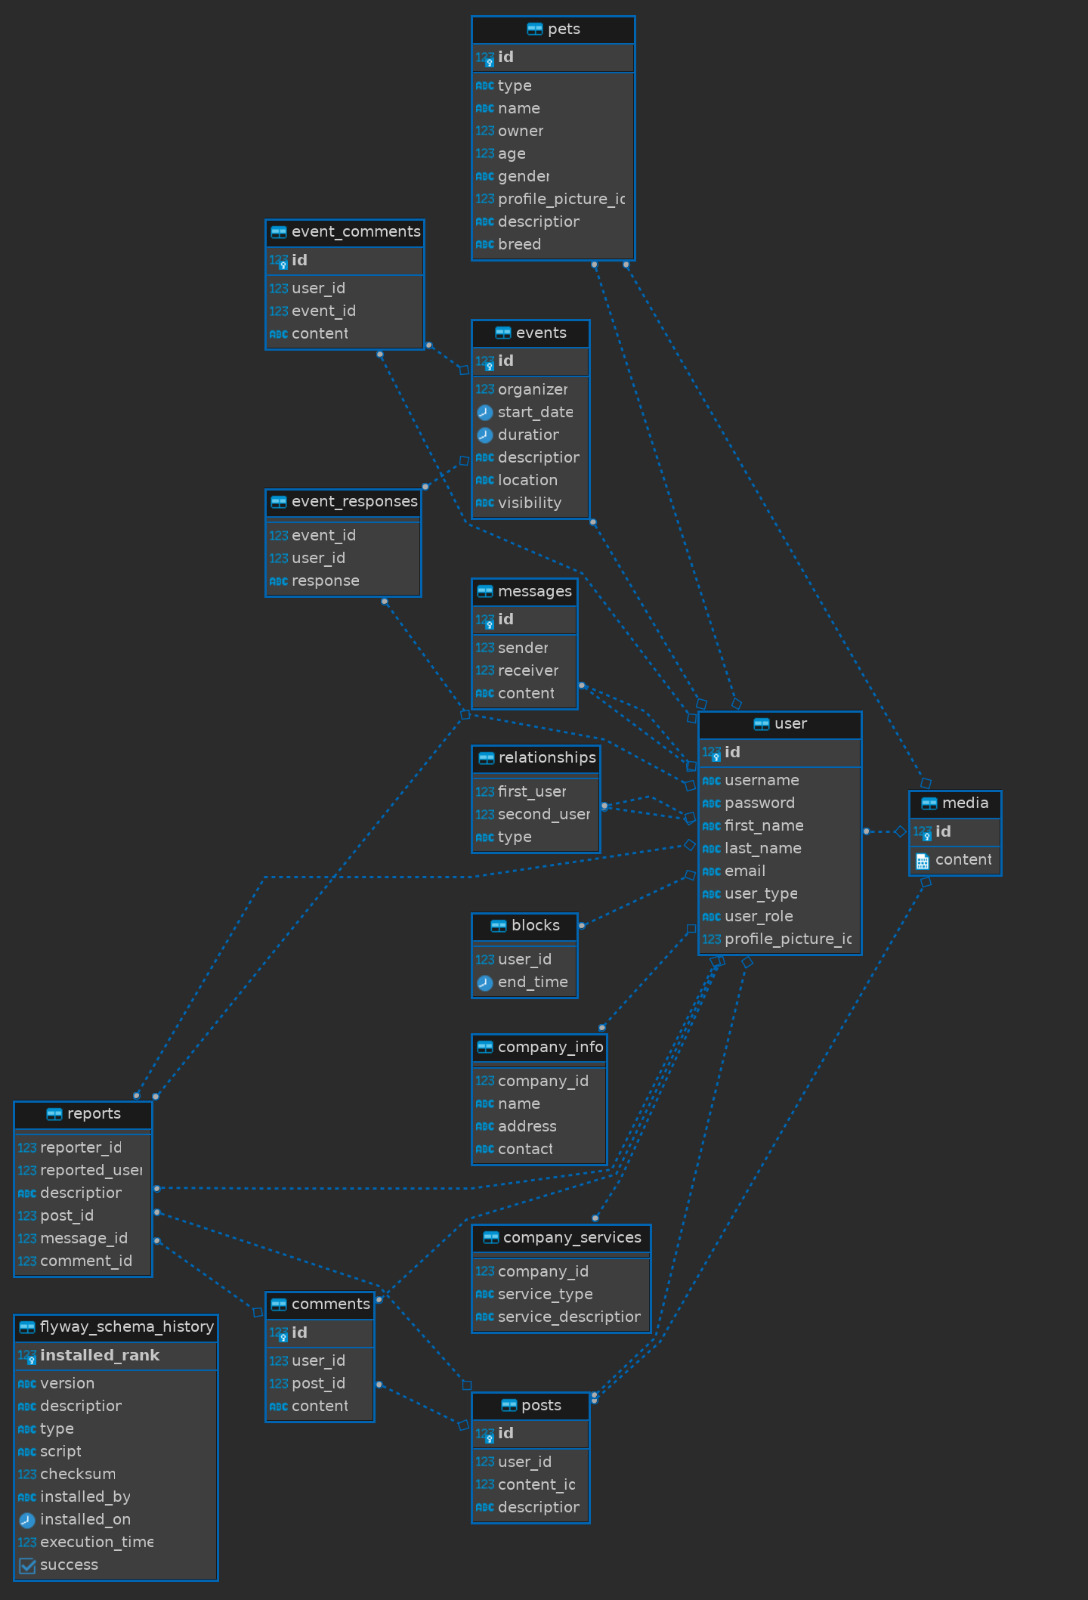
\includegraphics[scale = 0.37]{slike/dijagram_baze.jpeg}
					\centering
					\caption{Dijagram baze podataka}
					\label{fig:dijagram_baze}
				\end{figure}
			
			\eject
			
			
		\section{Dijagram razreda}
		
			Dijagram razreda prikazuje odnose izmedu različitih objekata, te njihove atribute
			i operacije kojima vladaju. Radi jednostavnosti, dijagram razreda je
			podijeljen u više slika.
			
			\begin{figure}[H]
				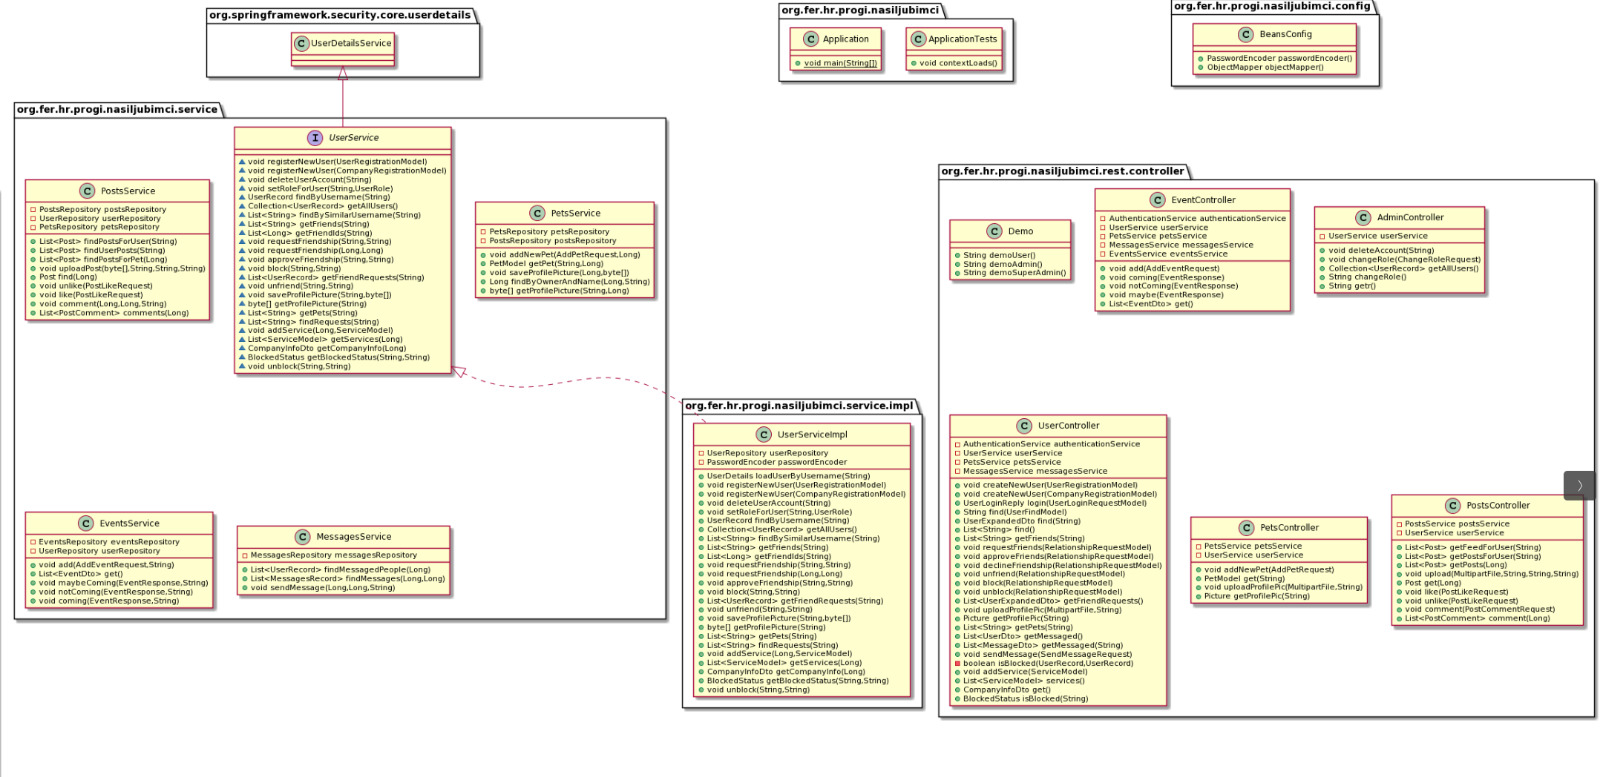
\includegraphics[scale=0.3]{slike/controller.jpeg} %veličina slike u odnosu na originalnu datoteku i pozicija slike
				\centering
				\caption{Dijagram razreda kontrolera}
			\end{figure}
		
			\begin{figure}[H]
				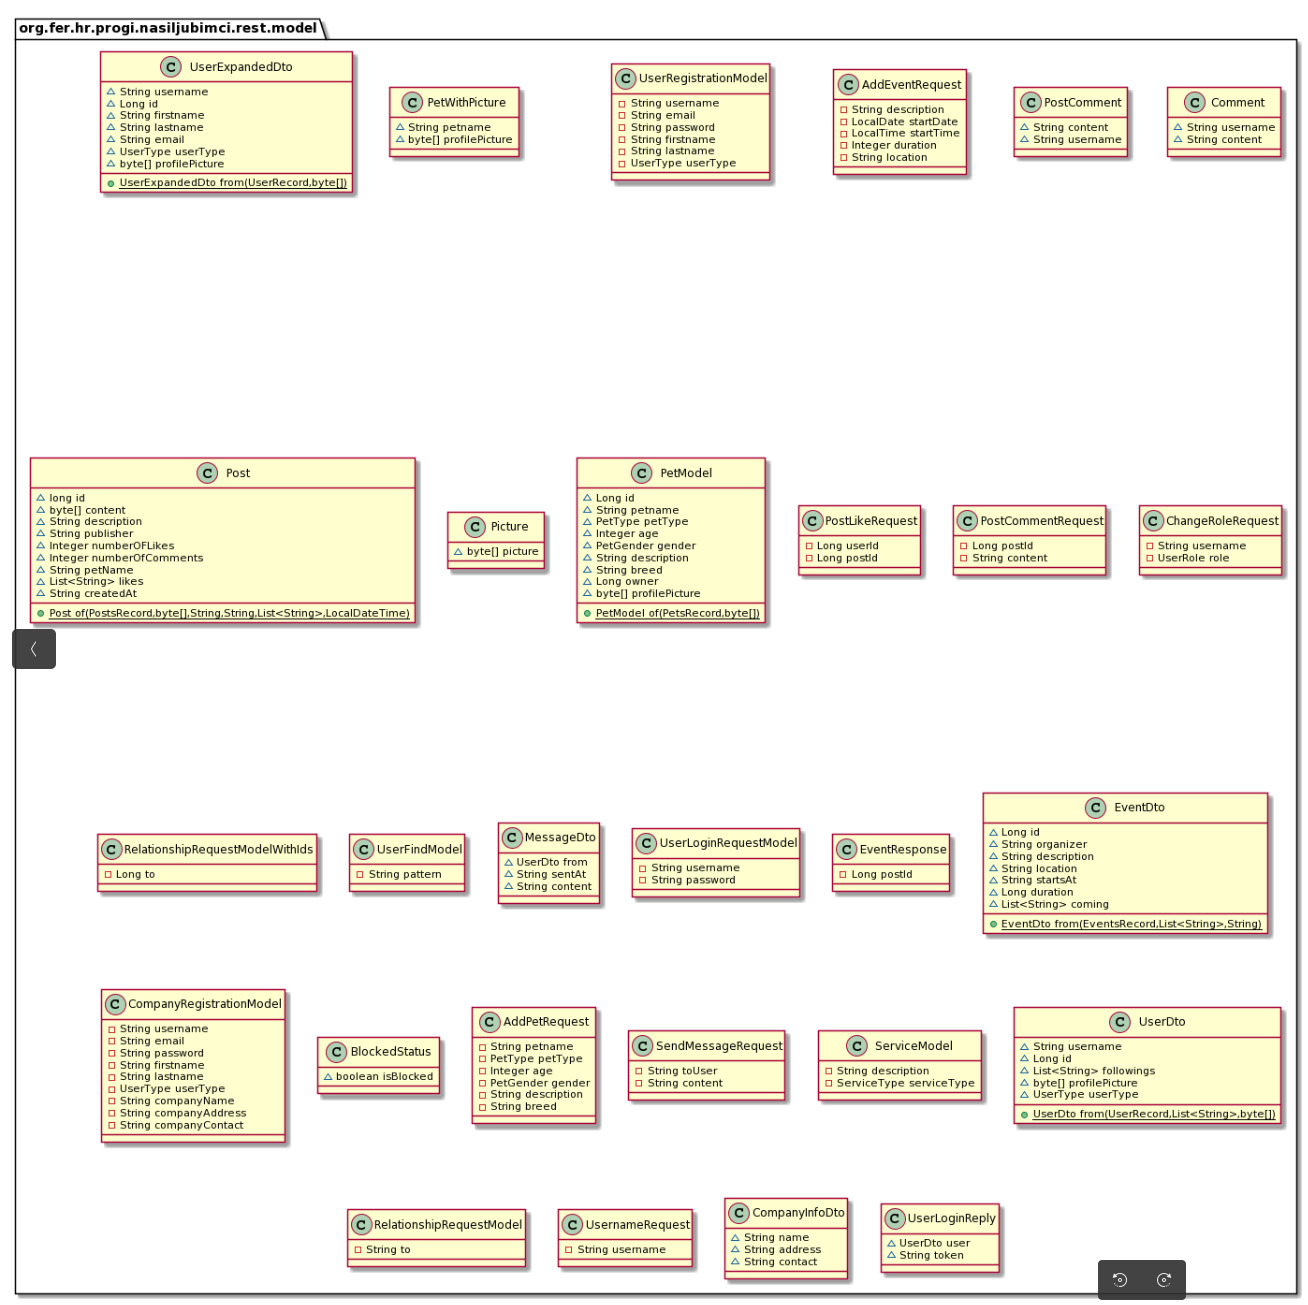
\includegraphics[scale=0.34]{slike/rest_model.jpeg} %veličina slike u odnosu na originalnu datoteku i pozicija slike
				\centering
				\caption{Dijagram razreda rest modela}
			\end{figure}
		
			\begin{figure}[H]
				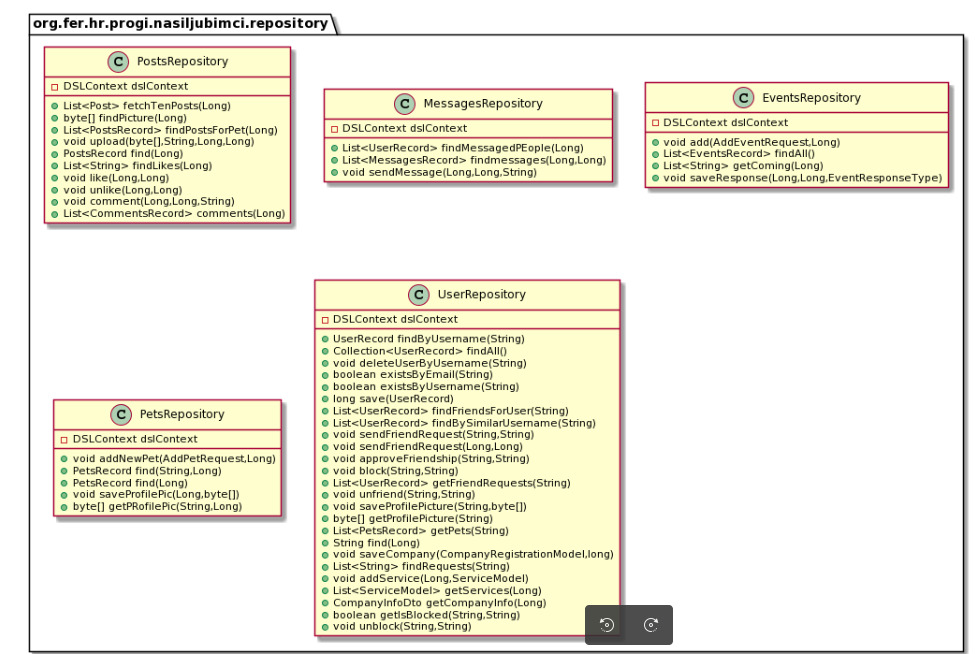
\includegraphics[scale=0.4]{slike/repository.jpeg} %veličina slike u odnosu na originalnu datoteku i pozicija slike
				\centering
				\caption{Dijagram razreda repozitorija}
			\end{figure}
		
			\begin{figure}[H]
				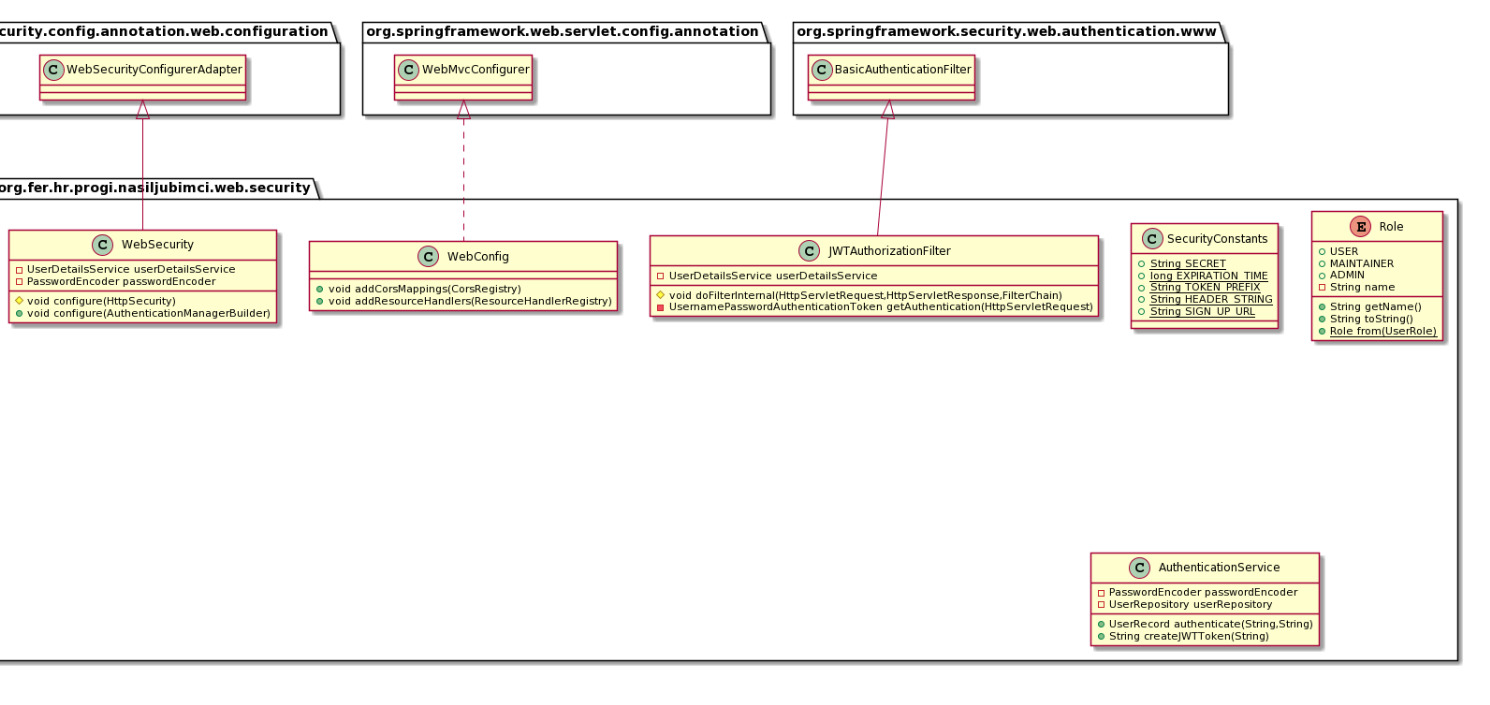
\includegraphics[scale=0.3]{slike/security.jpeg} %veličina slike u odnosu na originalnu datoteku i pozicija slike
				\centering
				\caption{Dijagram razreda securityja}
			\end{figure}
			
			
			\eject
		
		\section{Dijagram stanja}
			
			Dijagram stanja primjenjuje se za opis stanja objekta i za opisivanje prijelaza iz jednog u drugo stanje. Priložena slika prikazuje dijagram stanja objekta "Vlasnik". Vlasnik se prijavljuje u aplikaciju te nakon toga on prelazi u stanje "Početna stranica". S "Početne stranice" može prijeći na svoj "Osobni profil" odakle može izvršiti niz akcija. U završno stanje dolazi se nakon stanja "Početna stranica" i odjave iz aplikacije.
			\begin{figure}[H]
				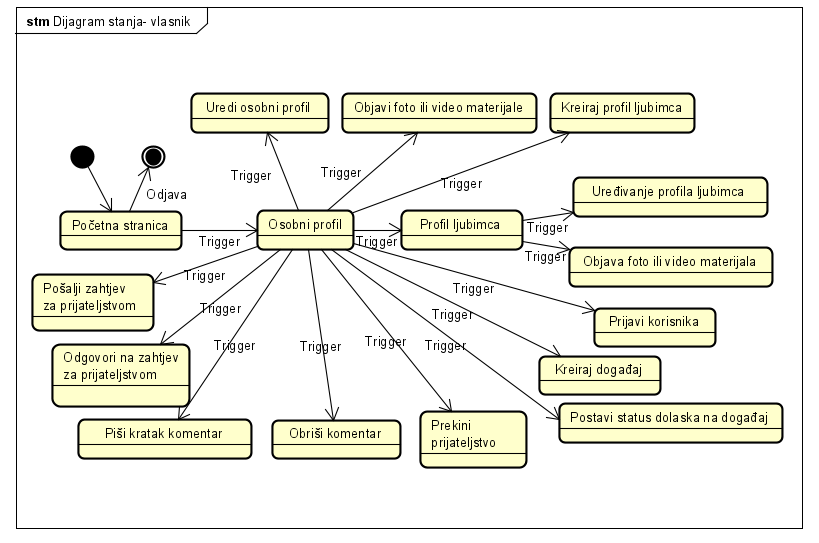
\includegraphics[width=\textwidth]{slike/Dijagram_stanja_vlasnik.png}
				\centering
				\caption{Dijagram stanja}
				\label{fig:classd_middle}
			\end{figure}
			
			
			\eject 
		
		\section{Dijagram aktivnosti}
			
			Dijagram aktivnosti prikazuje povezane aktivnosti na visokoj apstrakcijskoj razini. Dijagram aktivnosti intuitivno prikazuje kako podaci teku kroz aplikaciju i kako se kontrola nad podacima mijenja. Idući dijagram prikazuje proces prijave korisnika na neki od nadolazećih događaja.
			
			\begin{figure}[H]
				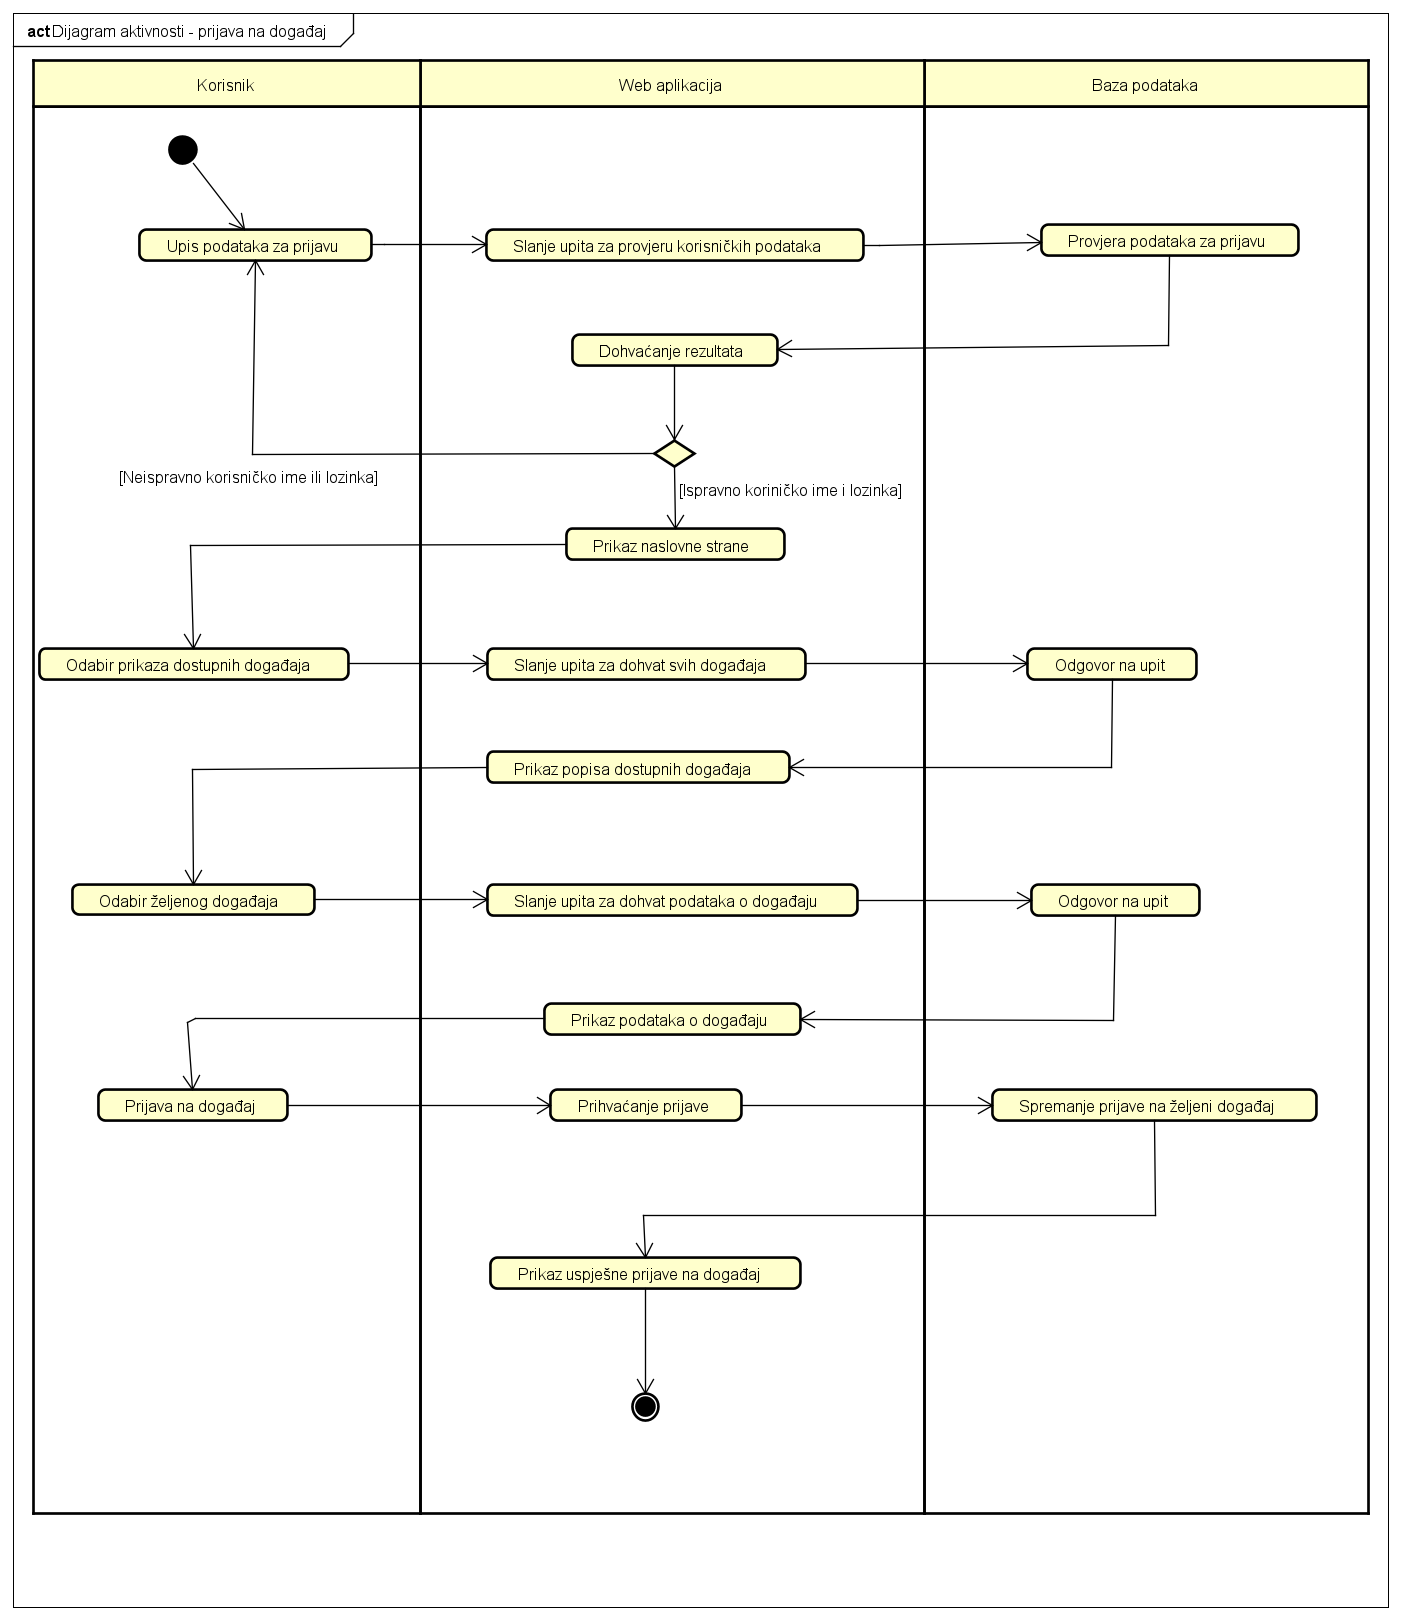
\includegraphics[width=\textwidth]{slike/Dijagram_aktivnosti.png}
				\centering
				\caption{Dijagram aktivnosti}
				\label{fig:classd_middle}
			\end{figure}
			
			\eject
		\section{Dijagram komponenti}
		
			\textbf{\textit{dio 2. revizije}}\\
		
			 \textit{Potrebno je priložiti dijagram komponenti s pripadajućim opisom. Dijagram komponenti treba prikazivati strukturu cijele aplikacije.}